\item \textbf{{[}ALVL/9597/2015/P2/Q4{]} }

An algorithm for converting a number n from denary to octal uses the
three built-in functions: 
\begin{center}
\begin{tabular}{|l|>{\raggedright}p{0.15\columnwidth}|>{\raggedright}p{0.25\columnwidth}|}
\hline 
\texttt{\hspace{0.01\columnwidth}}Function & \texttt{\hspace{0.01\columnwidth}}Description & \texttt{\hspace{0.01\columnwidth}}Example\tabularnewline
\hline 
\texttt{INTMOD(Number,Divisor)} & returns the remainder when the first parameter is divided by the second
parameter & \texttt{INTMOD(7,3) }returns 1\tabularnewline
\hline 
\texttt{INTDIV(Number,Divisor)} & returns the integer part when thefirst parameteris divided by the
second parameter. & \texttt{INTDIV(7,3) }returns 2\tabularnewline
\hline 
\texttt{SUBSTR(ThisString,Start,Length)} & forms a substring from ThisString, starting at Start (with first index
in string zero) and taking Length characters & \texttt{SUBSTR(``abcd'',1,2)} returns \texttt{``bc''}\tabularnewline
\hline 
\end{tabular}
\par\end{center}

Study the following pseudocode: 

\noindent %
\noindent\begin{minipage}[t]{1\columnwidth}%
\texttt{01 FUNCTION DenaryToOctal (n : INTEGER) RETURNS STRING }

\texttt{02 \qquad{}OctalDigits <- \textquotedbl 01234567\textquotedbl{} }

\texttt{03 \qquad{}IF n < 8 }

\texttt{04 \qquad{}\qquad{}THEN }

\texttt{05 \qquad{}\qquad{}\qquad{}TempString <- SUBSTR(OctalDigits,
n, 1) }

\texttt{06 \qquad{}\qquad{}ELSE }

\texttt{07 \qquad{}\qquad{}\qquad{}// '+' is the concatenation
operator }

\texttt{08 \qquad{}\qquad{}\qquad{}TempString <- DenaryToOctal(INTDIV(n,8))
+ SUBSTR(OctalDigits, INTMOD(n,8),1)) }

\texttt{09 \qquad{}ENDIF }

\texttt{10 \qquad{}RETURN TempString }

\texttt{11 ENDFUNCTION }%
\end{minipage}
\begin{enumerate}
\item Identify where and why this is a recursive function. \hfill{}{[}2{]}
\end{enumerate}
The diagram shows the execution of the call \texttt{DenaryToOctal(39)}. 
\begin{center}
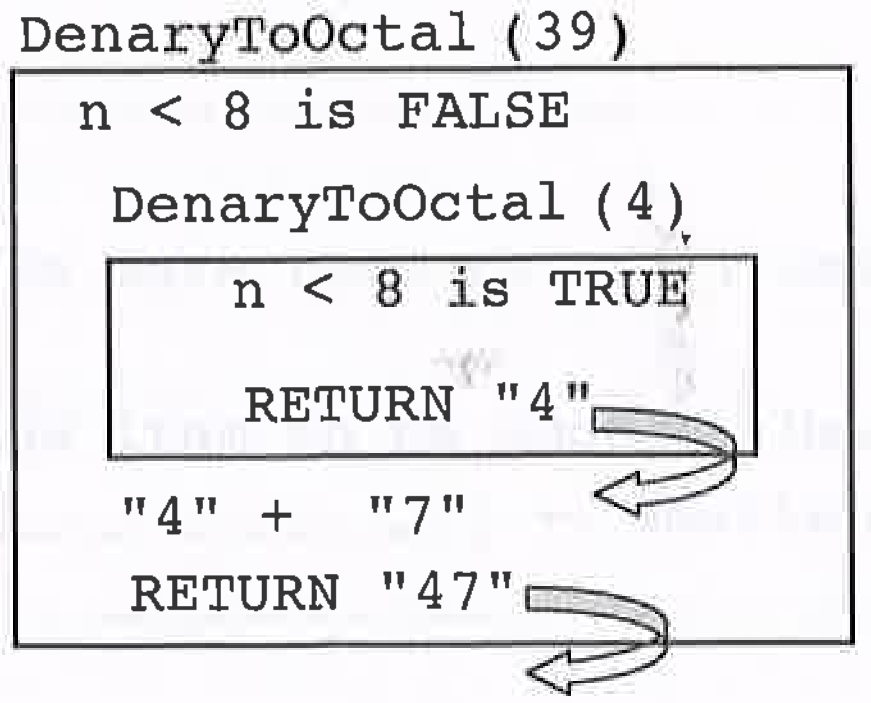
\includegraphics[width=0.5\paperwidth]{C:/Users/Admin/Desktop/Github/question_bank/LyX/static/img/9597-ALVL-2015-P2-Q4}
\par\end{center}
\begin{enumerate}
\item[(b)] Draw a similar diagram to show the execution of the call \texttt{DenaryToOctal(67)}.\hfill{}
{[}3{]}
\item[(c)] Changes are to be made to the function \texttt{DenaryToOctal()} so
that it converts denary numbers to hexadecimal.

Describe the changes: 
\begin{itemize}
\item that are essential to make the revised function work. 
\item that are non-essential but would help with the clarity of the pseudocode.\hfill{}
{[}5{]}
\end{itemize}
\end{enumerate}